\section{Naida, the Sea Nymph}

\begin{quotex}
\begin{verse}
While the nightingale sings,\\
both night and day,\\
I am with my beautiful\\
beneath the flowers,\\
until our sentry from the tower\\
cries: ``Lovers, get up!\\
for I clearly see the sunrise and the day.''
\end{verse}
\flright{\textit{Occitan Alba}}
\end{quotex}

\begin{wrapfigure}{rt}{.3\textwidth}
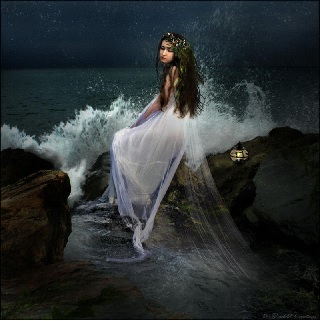
\includegraphics[width=.3\textwidth]{Nereid.jpg}
\end{wrapfigure}

As Naida was blossoming into womanhood, tales of her beauty began to circulate in the nearby villages. Many claimed that she had the gift of Second Sight. Her mother had died in childbirth, so Naida was raised in the forest with her father, the local healer. From him, she learned the secrets of the herbs of the countryside, which she would gather for her father's potions. He also taught her the mystic arts which had been passed down from father to son for generations. Without a male heir, he called her Niko, as it was the custom in that land to give the only child a boy's name.

The summers were spent by the sea. There Naida would go pearl diving, her hair yellowed by the Sun. When she suddenly appeared out of the sea, like some Nereid, the boys would rush to the shore just to gaze at her. They would retain that image all day until they tucked themselves under the sheets at night.

\paragraph{Axel}


One day, she heard the bad news. Her father had to leave to do battle with the Turanians invading from the East. He had a premonition that he would never return, so he arranged a marriage with an older man named Axel who lived in a northern country. Sadly, Naida left the only home she had ever known.

Axel was a prominent apothecary and spiritual counsellor, well respected in town. Since his business had been in decline, he relied on Naida to mix new herb combinations and on her scrying for spiritual counselling. Unfortunately, their marriage was more akin to a business arrangement than a work of love. Axel was as cold as the ocean wind that cut through her in winter and his soul as disharmonious as the sound of the language spoken in that land.

Naida could not even stand his touch and actually pushed him away on one fateful night. In fury, he exclaimed, ``If I can't have you, then no one can.'' He locked her in the upstairs room where she continued to mix herbs and scry for him. There was a small balcony overlooking the town square, from which she stared out all day. The men stopped, dazzled by her beauty, but the women could see the sadness in her eyes. Naida developed a network of women who would pass notes for her. In that way she communicated with the finest minds in Europe.

\paragraph{Arnaut}


One spring, the town was abuzz with rumours that the famous Troubadour Arnaut would be passing through. Some even said that he learned the secret teachings of the Templars from his grandfather who had fought alongside the Knights in the Second Crusade. Arnaut would meet with his followers in different towns and villages as he travelled.

Even Naida could not conceal her glee when she heard the news. Arnaut was handsome, refined, wise, and romantic; all the qualities that the young Naida had dreamed of in a man, yet evaded her in her maturity.

Arnaut did not disappoint. Every afternoon, he would set up in the town centre. Sometimes with a lute, other times with a hurdy-gurdy, he would sing songs of love, betrayal, infidelity, and the exploits of famous Knights. There would occasionally be satires about the foibles of the ruling classes.

Even Arnaut, despite his sophistication, was smitten by Naida who watched him sing from above. During the performance of one particular Alba\footnote{\url{https://en.wikipedia.org/wiki/Alba\_(poetry)}}, he felt a tear fall from the balcony, which burned into his skin like a drop of caustic acid. He resolved that Naida should never again shed such a tear. Gossipers claimed that Arnaut was composing new songs just for Naida.

\paragraph{Courtly Love}


At first, they communicated by her system of notes. Later, his students would set up a ladder so he could speak to her through the bars of the balcony after the lamplights were extinguished. They would talk through the night, about their lives, their dreams, and more often of their deepening love. More importantly, they would discuss the Hermetic sciences. Naida passed her father's extensive notes onto Arnaut, so they would never be lost. These were the same teachings that Dante learned during his travels on the that side of the Adriatic Sea.

Arnaut's students would return to warn him of the approaching dawn, which signalled another painful separation. Arnaut's days continued: Singing in the afternoon, clandestine meetings with his students at dusk, then stolen moments of furtive joy at night with Naida.

\paragraph{The Test}


During one fateful meeting, which was destined to be their last, Naida told Arnaut that she needed some herbs grown only in Latvia. Her husband was getting suspicious and made the odd request. Not wishing to be punished again, she pleaded with Arnaut to fulfil that request.

On his return from the difficult journey to Latvia, several students rushed outside the city gates to warn Arnaud not to enter. Axel had convinced the authorities that Arnaut was teaching heresy. Not only was his life in danger, but so were those of the students if he entered. And Naida might be tried as a witch.

Greatly distressed, Arnaut turned back and resumed his meanderings, singing in town squares, and meeting secretly with his students across Europe. Occasionally, he would receive a perfumed note from Naida, pledging her undying love. The last missive was a tear soaked sheet of paper with no note. Arnaut understood at once that he had failed his pledge that Naida would never shed another tear.

Naida was let out of her room and she accepted her position as a prominent woman in the town.

Although Arnaut visited many more towns, and met many more women, he was never able to love again. Some say that, in recompense, his most beautiful, yet poignant, songs were composed during this period.

\begin{quotex}
During the lockdown, I set myself the challenge to write stories like the ones in the Decameron by \textbf{Giovanni Boccaccio}, with a hidden message. His book of stories was also written during an epidemic. This is one of the stories for the \emph{New Decameron}.
\end{quotex}



\flrightit{Posted on 2020-09-01 by Anonymous}

